\documentclass{article}
\usepackage{graphicx} % Required for inserting images

\usepackage[a4paper, left=1.5cm, right=1.5cm, top=1cm, bottom=2cm]{geometry}

\usepackage{float}

\newcounter{commentCount}
\newcounter{filePrg}
\newcounter{inputPrg}

\usepackage[dvipsnames]{xcolor}
\usepackage{minted}

\usepackage[many]{tcolorbox}
\tcbuselibrary{listings}
\tcbuselibrary{minted}

\usepackage{ifthen}
\usepackage{fontawesome}

\usepackage{tabularx}
\newcolumntype{\CeX}{>{\centering\let\newline\\\arraybackslash}X}%
\newcommand{\TwoSymbolsAndText}[3]{%
  \begin{tabularx}{\textwidth}{c\CeX c}%
    #1 & #2 & #3
  \end{tabularx}%
}

\newtcblisting[use counter=inputPrg, number format=\arabic]{codeInput}[4]{
  listing engine=minted,
  minted language=#1,
  minted options={autogobble,breaklines,  firstnumber={#4}},
  listing only,
  size=title,
  arc=1.5mm,
  breakable,
  enhanced jigsaw,
  colframe=myblue,
  coltitle=White,
  boxrule=0.5mm,
  colback=white,
  coltext=Black,
  title=\TwoSymbolsAndText{\faCode}{%
  \textbf{Sql Program \thetcbcounter}\ifthenelse{\equal{#2}{}}{}{\textbf{: }#2}%
  }{\faCode},
  label=inputPrg:#3
}


\usepackage{boldline}
\usepackage{tikz,tcolorbox}
\usepackage{amsmath}
\usepackage[table,xcdraw]{xcolor}
\usepackage{listings}
\usepackage{array,multirow} % For customizing tables
\usepackage{booktabs} % For better horizontal lines
\usepackage{makecell}
\setlength{\parindent}{0pt}
\usepackage{siunitx}
\usepackage{tkz-tab}
\usepackage{amssymb}
\usepackage{amsmath}
\usepackage{enumitem}

\usepackage{caption}
\usepackage{float}


\newcommand{\exer}[1]{
  \section*{Exercice #1}
  \vspace{-0.5cm}
  \noindent\rule{\textwidth}{0.5pt}%
}

\newcommand{\tit}[1]{
\begin{center}
    \Large{\textbf{{#1}}}
\end{center}
}

\definecolor{commentgray}{HTML}{676160}
\definecolor{messagegreen}{HTML}{17B867}
\definecolor{myblue}{HTML}{10C2C4}

\tcbuselibrary{skins, breakable, theorems}


\newtcolorbox{prettyBox}[2]{
  enhanced,
  colback=white!90!#2,   % Background color based on the second parameter (color)
  colframe=#2!60!black,  % Frame color based on the second parameter (color)
  coltitle=white,        % Title color (white)
  fonttitle=\bfseries\Large,
  title=#1,              % Title from the first parameter
  boxrule=1mm,
  arc=0.5mm,
  drop shadow=#2!35!gray, % Drop shadow color based on the second parameter (color)
}

\usepackage{hyperref}
\hypersetup{
    colorlinks=true,
    linkcolor=blue,
    filecolor=magenta,      
    urlcolor=cyan,
    pdftitle={Overleaf Example},
    pdfpagemode=FullScreen,
    }



\lstdefinestyle{cmd}{
 basicstyle=\ttfamily,
 backgroundcolor=\color{lightgray!20},
 frame=single
}
\usepackage{subcaption}
\usepackage{minted}

\begin{document}

\tit{How To Install MongoDB}

\vspace{0.5cm}

\section{Install MongoDB Server}
\begin{prettyBox}{MongoDB Server}{myblue}
    \begin{itemize}
        \item Download the server using this link : \href{https://fastdl.mongodb.org/windows/mongodb-windows-x86_64-8.2.5-signed.msi}{https://fastdl.mongodb.org/windows/mongodb-windows-x86_64-8.2.5-signed.msi}
        \item Run the msi and choose complete installation
        \item Make sure to remember the path where service is installed it's important for later to set environment variable for the bin.
        \item check mongo compass.
        \item Installation will start.
    \end{itemize}
   
\end{prettyBox}

\section{Install Mongo Shell}
\begin{prettyBox}{MongoDB Service}{myblue}
    \begin{itemize}
        \item Download the shell using this link : 
\href{https://downloads.mongodb.com/compass/mongosh-2.7.0-win32-x64.zip}{https://downloads.mongodb.com/compass/mongosh-2.7.0-win32-x64.zip} 
       \item unzip it and make sure to remember where you unziped it's important for later to set environment variable for the bin.
    \end{itemize}
\end{prettyBox}


\begin{figure}[H]
  \begin{subfigure}[H]{.4\textwidth}
    \centering
    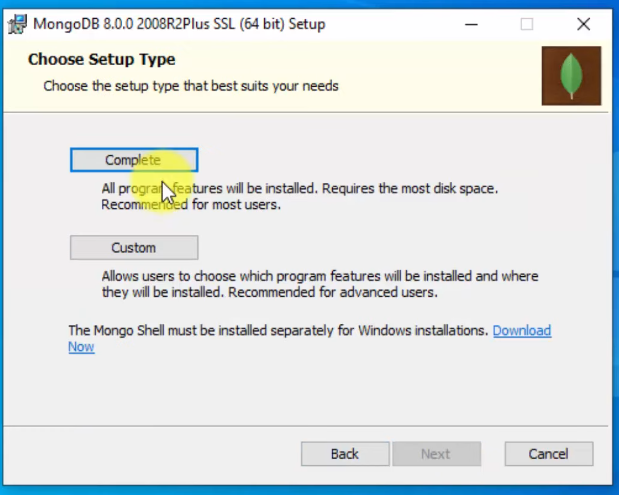
\includegraphics[width=\linewidth]{complete.png}
    \caption*{Choose Complete Installation}
  \end{subfigure}
  \hfill
  \begin{subfigure}[H]{.4\textwidth}
    \centering
    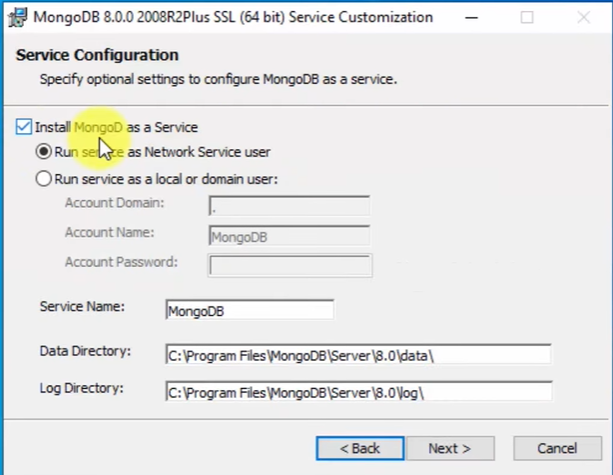
\includegraphics[width=\linewidth]{path.png}
    \caption*{Choose Path}
  \end{subfigure}

  \medskip

  \begin{subfigure}[H]{.4\textwidth}
    \centering
    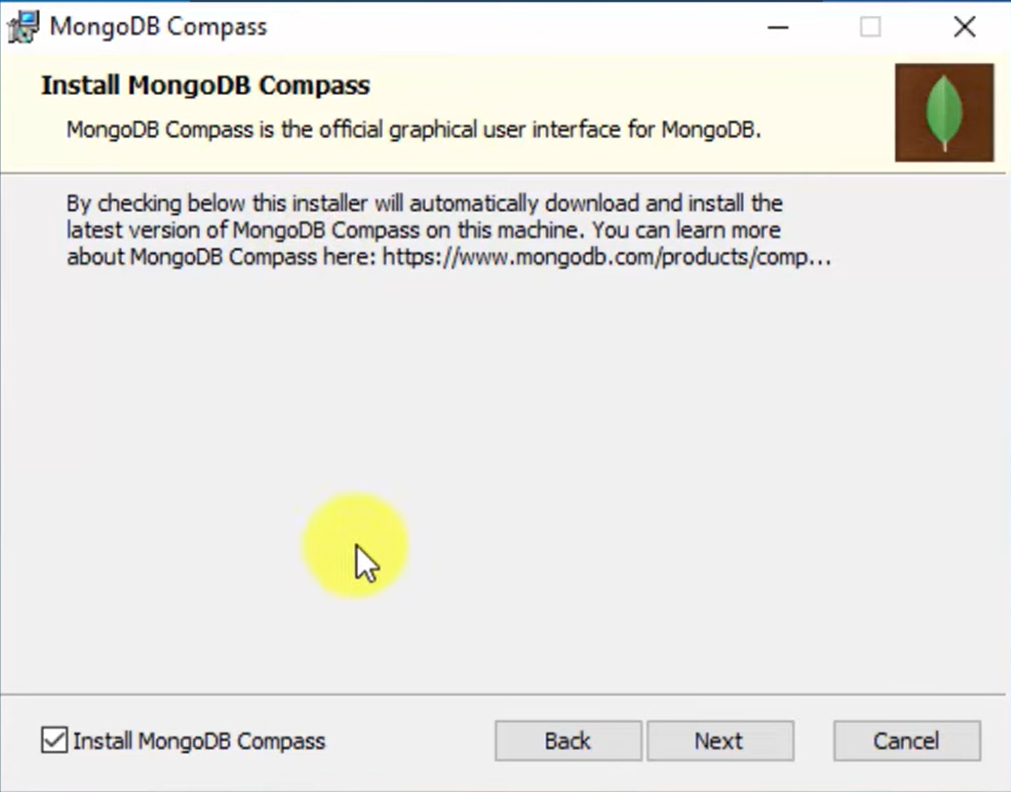
\includegraphics[width=\linewidth]{checked.png}
    \caption*{checking MongoDB Compass}
  \end{subfigure}
  \hfill
  \begin{subfigure}[H]{.4\textwidth}
    \centering
    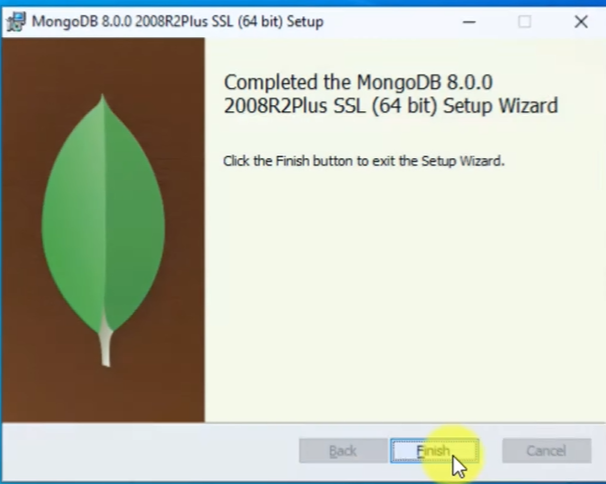
\includegraphics[width=\linewidth]{finish.png}
    \caption*{Finished}
  \end{subfigure}
\end{figure}



\section{Set Up Environment Variables}
\begin{prettyBox}{Environment Variables}{myblue}
You need to add 2 Environment Variables one for the server and the other for the shell inside the system variable \texttt{Path}
\end{prettyBox}

\vspace{0.25cm}
\begin{figure}[H] 
  \centering 
  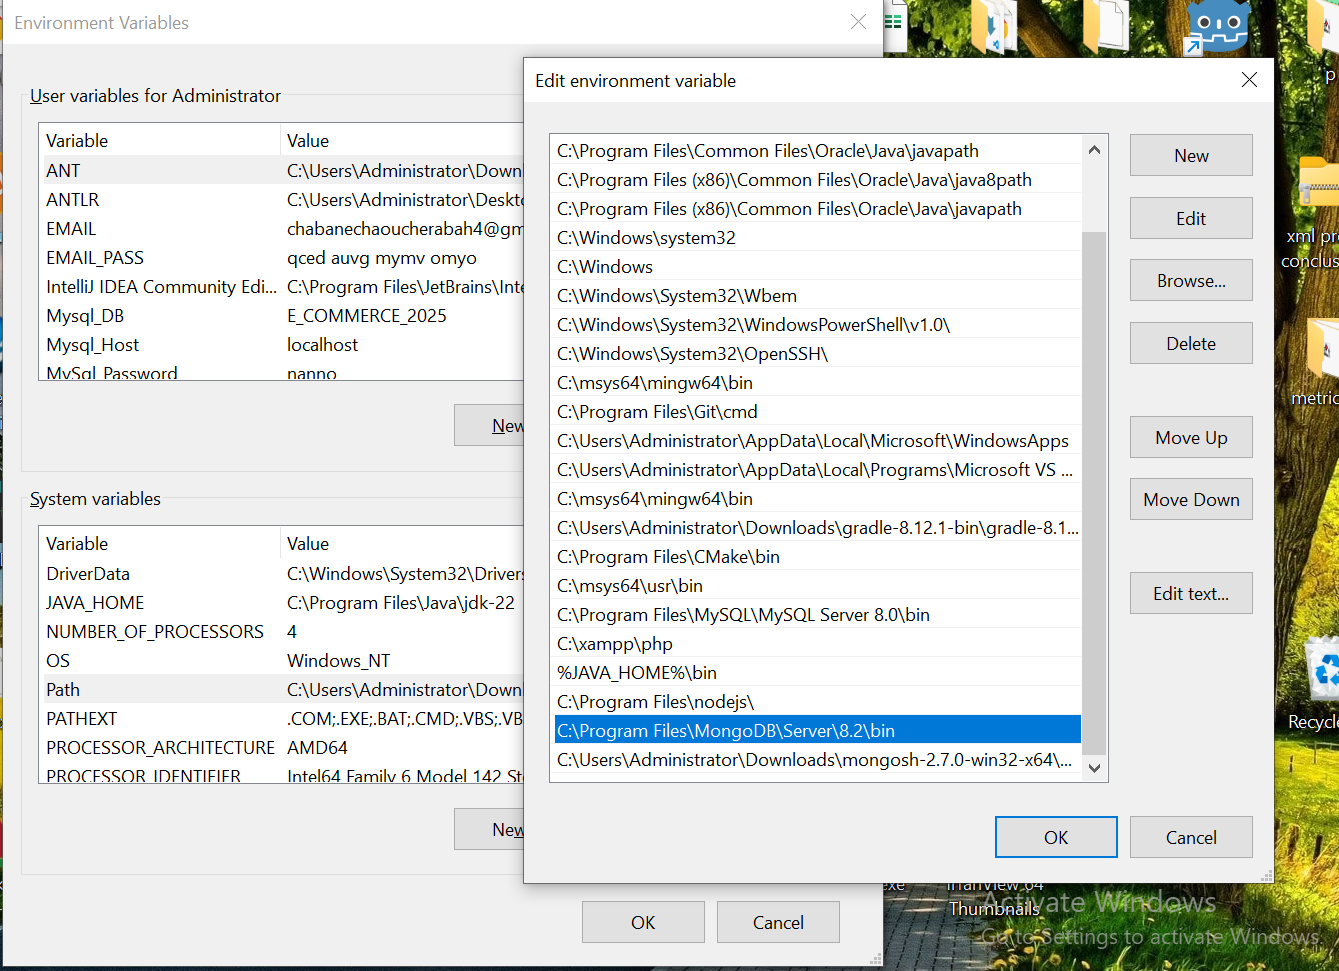
\includegraphics[width=0.8\textwidth]{env.png} 
\end{figure}




\section{Verification}
\begin{prettyBox}{Verification}{myblue}
in the command line (cmd) we will run the following commands :
\begin{itemize}
    \item \texttt{mongod --version} to check if the server exist.
    \item \texttt{mongosh} to use the mongo shell.
\end{itemize}
\end{prettyBox}



\vspace{0.25cm}
\begin{figure}[H] 
  \centering 
  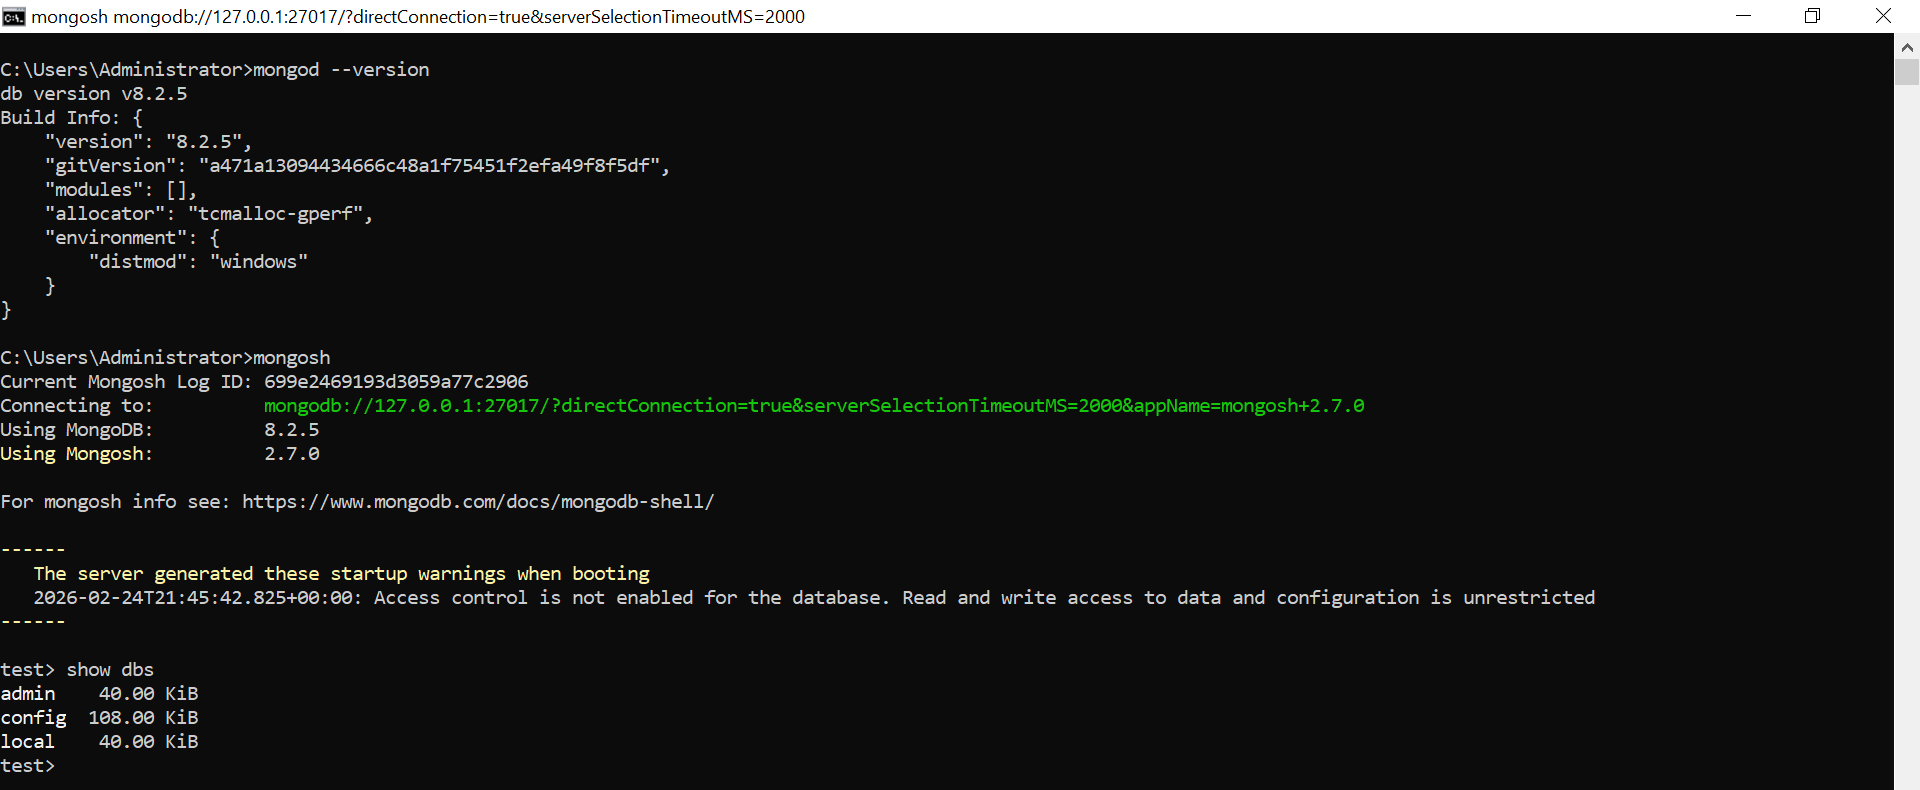
\includegraphics[width=0.8\textwidth]{cmd.png} 
\end{figure}


\end{document}
